\documentclass{elbioimp2}
\usepackage[utf8]{inputenc}

\usepackage[backend=biber,style=vancouver]{biblatex}
\usepackage{csquotes}

\title{Aerodynamics of a wedge shaped vehicle: Tesla cybertruck}
\author{\textbf{Federico Cutolo}\affiliation{Department of Aerospace Science and Technology, Politecnico di Milano, Milano, Italy}, E. Monti, G. J. Basile, E. Capone\affiliation{Department of Mechanics, Politecnico di Milano, Milano, Italy}} 

 
\addbibresource{demo.bib}

\begin{document}
\maketitle
\begin{abstract}
  Drag coefficient is assessed for different vehicle configurations through Computational Fluid Dynamics (CFD) analysis using OpenFOAM\textsupercript\textregistered. Data validation is carried out with experimental testing in wind tunnel. The  range of tested velocities is between 5 and 20 $m/s$. The experimental results show agreement with CFD analysis: an error of 14,2\% between the two is observed. The low values of the drag coefficient are due to the flow reattachment performed by vortexes generated at the A and C pillars.
  \keywords{Cybertruck, CFD; aerodynamics; vortexes; flow reattachment}
\end{abstract}
\section{Introduction}
The automotive industry is continuously developing new electrified power-train and vehicle architectures in order to optimize fuel consumption and reduce carbon dioxide emissions.
One of the most significant Key Performance Indicators for full-electric vehicles is the range covered by a full charge of the batteries. Therefore, the minimization of the aerodynamic resistance plays a critical role. 

\section{Targets and Methodology}
The workflow could be summed up as follows:
\begin{itemize}
    \item $C_x$ assessment for three vehicle configurations (CFD, experimental)
    \item $C_m$ sensitivity to crosswind conditions (experimental)
    \item $C_x$ sensitivity to ground-clearance (experimental)
    \item Full-scale and scaled model comparison (CFD)
    \item 3D characterization of the flow (CFD, experimental)
    \item Energy consumption sensitivity to $C_x$ (WLTP theoretical)
\end{itemize}


\section{Geometry modeling}
The Tesla Cybertruck is a concept pickup truck whose cargo area can be completely closed by means of an electric sunroof. The open cargo will be named as \emph{pickup}, while the closed one as \emph{sloped}. Nevertheless, an additional made-up configuration will be considered, in order to further investigate the influence of the tail shape in the aerodynamics of the truck. It will be named \emph{wagon}. The CAD has been built based on both official and non-official sources, such as blueprints from Tesla website and enthusiasts forums.
\begin{figure}[htp]
  \centering
  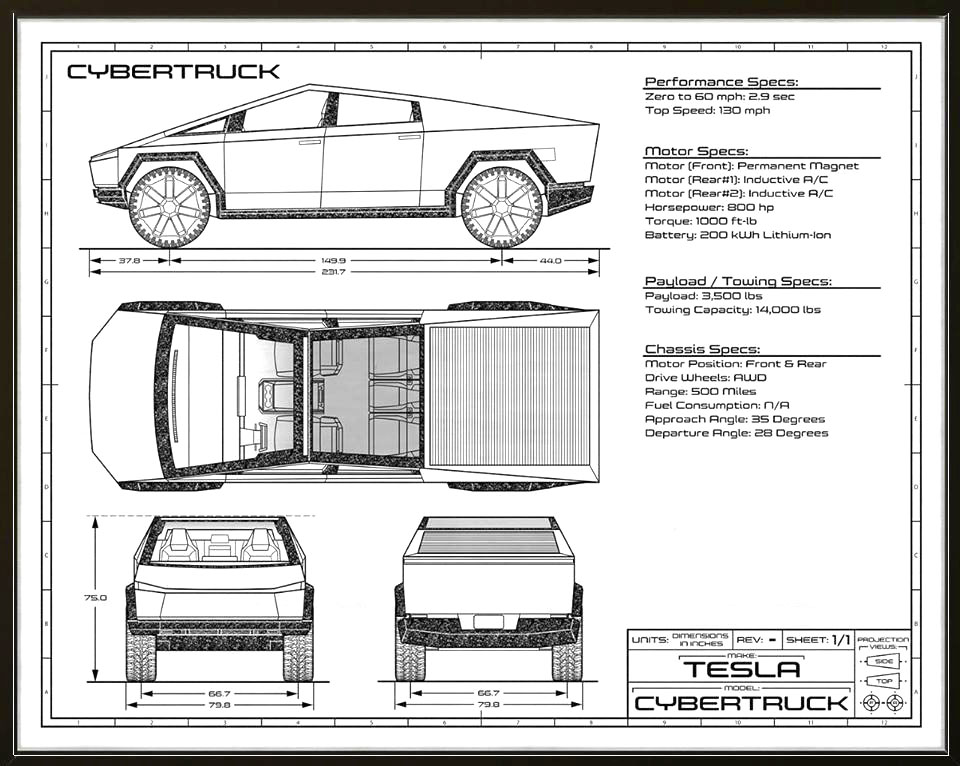
\includegraphics[width=0.9\columnwidth]{blueprint}
  \caption{Tesla Cybertruck blueprint.\label{Blueprint}}
\end{figure}

\section{CFD}
CFD analysis was lead for full-scale and wind-tunnel-scaled cases in order to obtain a more reliable comparison with the real world and the wind tunnel environment. The software used is OpenFOAM, hence the following procedure and terms are referred to it. For the sake of briefness, the \emph{Sloped} configuration is considered henceforth. 
\subsection{Expectations}
Due to the sharply-cornered design of the car, the expectation was to observe many flow separations, thus poor performance of the vehicle. A 2D analysis supported this hypothesis: the flow separated at the corners independently from the velocity, leading to a poor pressure recovery along the vehicle. 
\begin{figure}[htp]
  \centering
  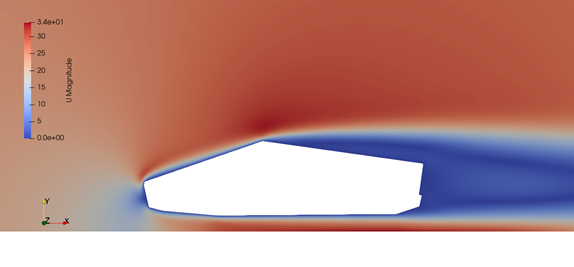
\includegraphics[width=0.9\columnwidth]{2d.png}
  \caption{Flow separation across the edges, 2D case.\label{}}
\end{figure}

\subsection{Domain}
At first, the whole-body model was analysed. However, due to the visible symmetry in the flow ~\ref{full-half comparison}, a halved body model was then considered. Thanks to this, a much greater amount of cells could be achieved at given computational resources.
\begin{figure}[htp]
  \centering
  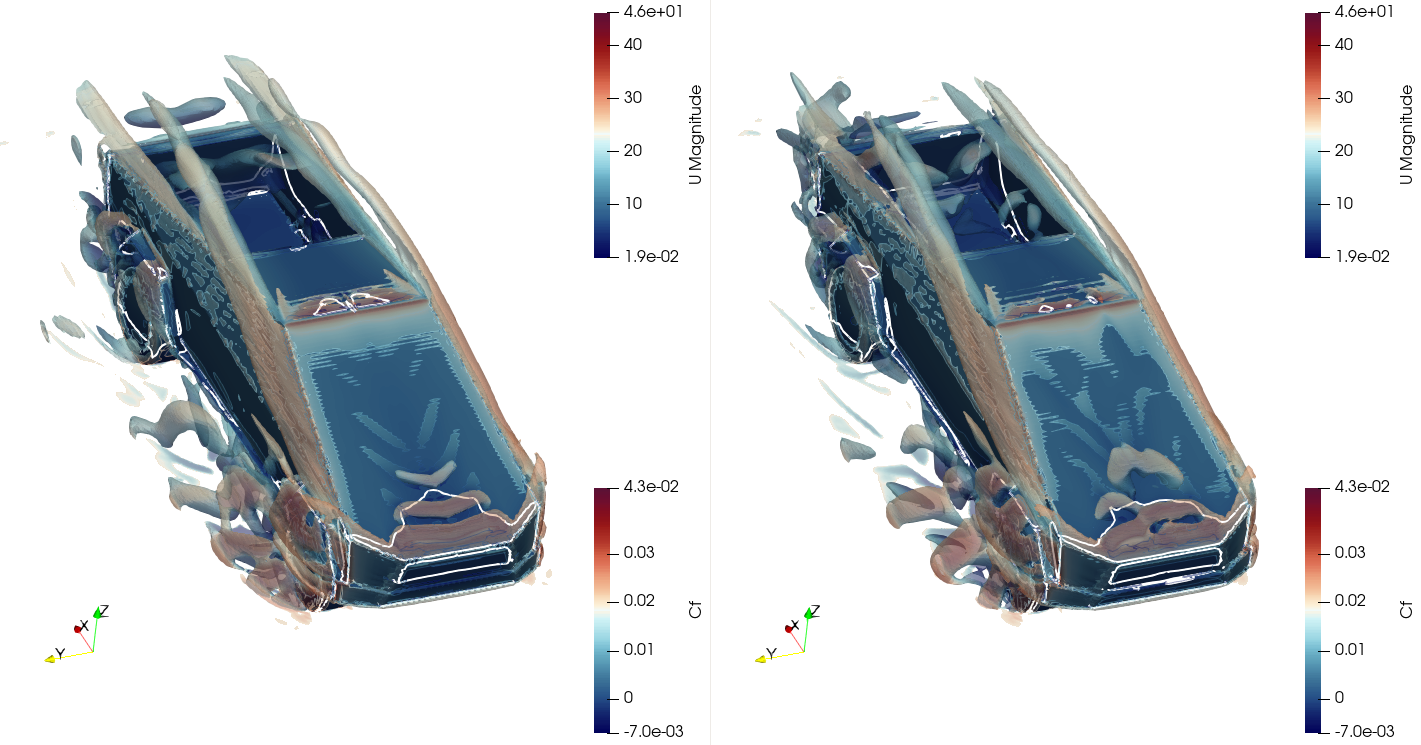
\includegraphics[width=0.9\columnwidth]{fullhalf.png}
  \caption{Whole-body and half-body show similar flow structures.\label{full-half comparison}}
\end{figure}
The computational domain for the full-scale case had to account for blockage ratio and boundaries effects minimization. For these reasons,  the inlet was placed two car-lengths in front, the outlet four car-lengths behind, while four cars-widths from the vehicle were taken for side walls. The floor was raised to intersect the wheels to reproduce the tyre patch, thus the actual ride height. The upper wall was placed at four car-heights afar from the vehicle roof.
On the other hand, the scaled domain had to observe the wind tunnel dimensions.\\ \noindent


\begin{tabular}{|l|r|r|r|}
\hline
                & L [$m$]       & H [$m$]   & W [$m$]   \\
\hline
Full-scale      & 8             & 40        & 16        \\
Wind tunnel     & 1             & 0.5       & 0.5       \\
\hline
\end{tabular} \\ 

\subsection{Mesh}

\subsubsubsection{Refinement boxes.}
The first step was to find the wake, separation and vortexes influence regions. That was managed with trial-and-error approach: step by step, where the grid refinement didn't affect the flow development, refinement boxes were put closer and tighter to the car ~\ref{boxes}
\begin{figure}[htp]
  \centering
  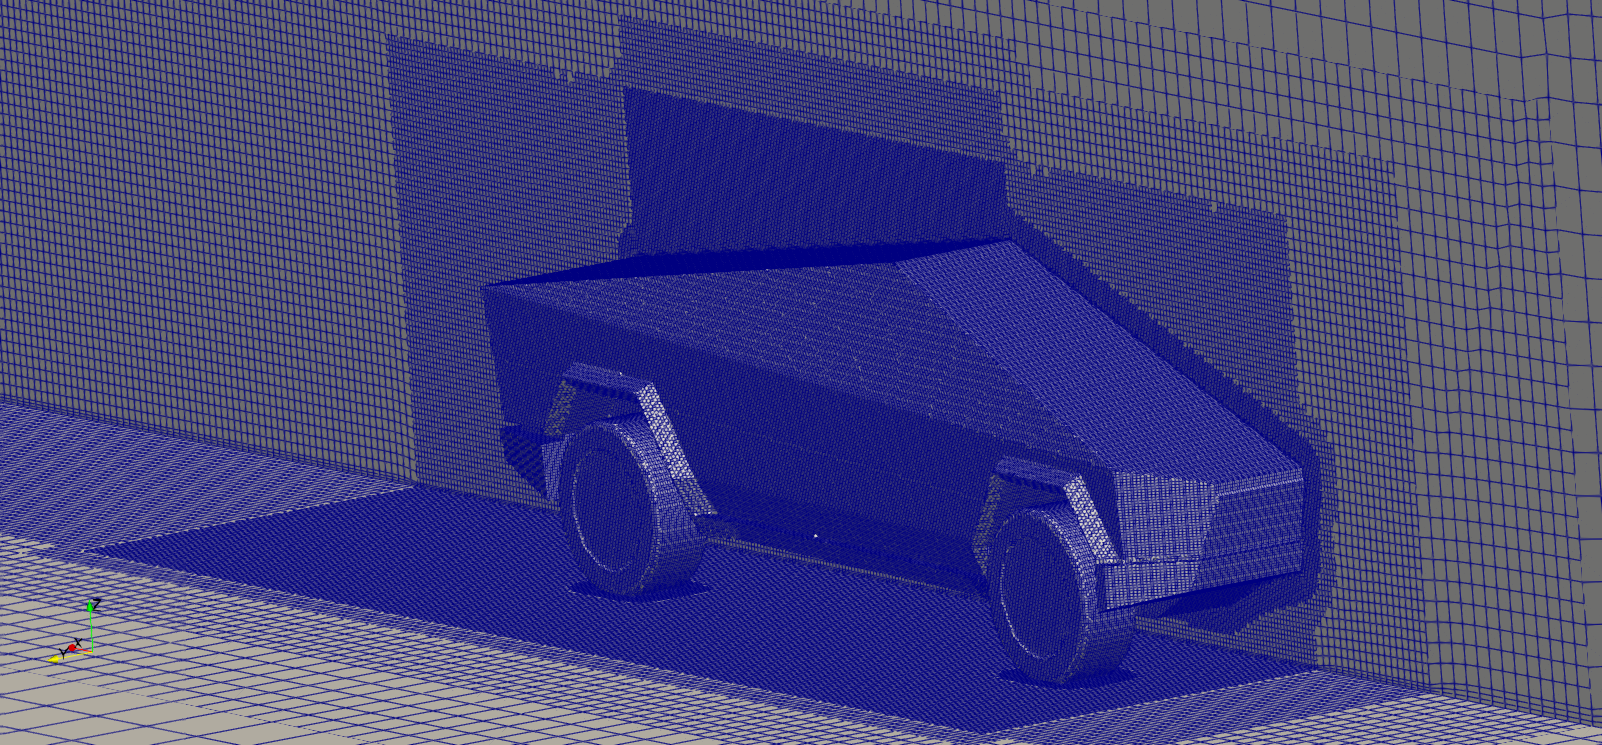
\includegraphics[width=0.9\columnwidth]{boxes.png}
  \caption{Refinement boxes around the car.\label{boxes}}
\end{figure}

\subsubsubsection{Boundary layer.}
For both the full-scale and scaled domains mesh layers were placed at surface of the body. However, to reproduce the ground of the test section of the wind tunnel, the scaled domain needed another layer on the lower wall.
\subsubsubsubsection{Mesh convergence}
In order to ensure the independence of the results from the mesh size, a mesh convergence study has been lead. The convergence is obtained around four million elements ~\ref{convergence}.A negligible difference in the $C_x$ is achieved for more cells, thus the previous dimension of the mesh was chosen.

\begin{figure}[htp]
  \centering
  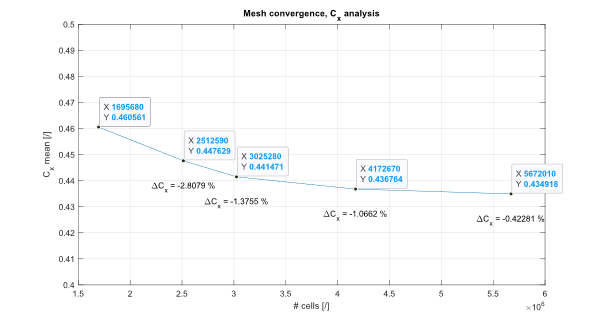
\includegraphics[width=0.9\columnwidth]{covergence.png}
  \caption{Mesh convergence with respect to $C_x$ for the \emph{Sloped} configuration.\label{convergence}}
\end{figure}

\subsection{Boundary conditions}
Turbulent quantities were estimated with a NASA database tool, considering a turbulence intensity of 5\%. (http://www.wolfdynamics.com/tools.html?id=110)\\

\begin{tabular}{|l|r|r|r|}
\hline
\multicolumn{4}{|c|}{\textbf{Full-scale domain (25 m/s)}} \\
\hline
\textbf{Patch} & \textbf{U} & \textbf{p} & \textbf{Turbulence} \\
\hline
\textbf{Body} & noSlip & zeroGrad. & wallFun. \\
\textbf{Wheels} & rotat.WallVel & zeroGrad. & wallFun. \\
\textbf{Inlet} & fixedValue & zeroGrad. & fixedValue \\
\textbf{Outlet} & intetOutlet & fixedValue & inletOutlet \\
\textbf{Lower wall} & fixedValue & zeroGrad. & wallFun. \\
\textbf{Median Plane} & symmetry & simmetry & symmetry \\
\textbf{Back wall} & slip & slip & slip \\
\textbf{Upper wall} & slip & slip & slip \\
\hline
\end{tabular} \\

\begin{tabular}{|l|r|r|r|}
    \hline
    \multicolumn{4}{|c|}{\textbf{Wind tunnel domain (20 m/s)}} \\
    \hline
    \textbf{Patch} & \textbf{U} & \textbf{p} & \textbf{Turbulence} \\
    \hline
    \textbf{Body} & noSlip & zeroGrad. & wallFun. \\
    \textbf{Wheels} & noSlip & zeroGrad. & wallFun. \\
    \textbf{Inlet} & pres.In.Vel & totalPres. & fixedValue \\
    \textbf{Outlet} & pres.In.Out.Vel & totalPres. & inletOutlet \\
    \textbf{Lower wall} & noSlip & zeroGrad. & wallFun. \\
    \textbf{Median Plane} & symmetry & simmetry & symmetry \\
    \textbf{Back wall} & noSlip & zeroGrad. & wallFun. \\
    \textbf{Upper wall} & noSlip & zeroGrad. & wallFun. \\
    \hline
\end{tabular}\\

\subsection{Results}
As expected, flow separation takes place at the sharp corners of the car, and high-pressure regions are identified just in front of them. 
The following drag coefficients are obtained.\\

\begin{tabular}{|l|r|r|r|}
\hline
$C_x$               & Pickup            & Sloped        & Wagon   \\
\hline
Full-scale          & 0.440             & 0.435         & 0.502    \\
Wind tunnel         & 0.512             & 0.489         & 0.549       \\
\hline
\end{tabular}\\

It is possible to observe two couples of longitudinal vortexes originating by the A-pillar and C-pillar ~\ref{vortexes}. The coupled vortexes are counter-rotating, hence they don't coalesce, and move closer to the centre of the roof along the vehicle. 
\begin{figure}[htp]
  \centering
  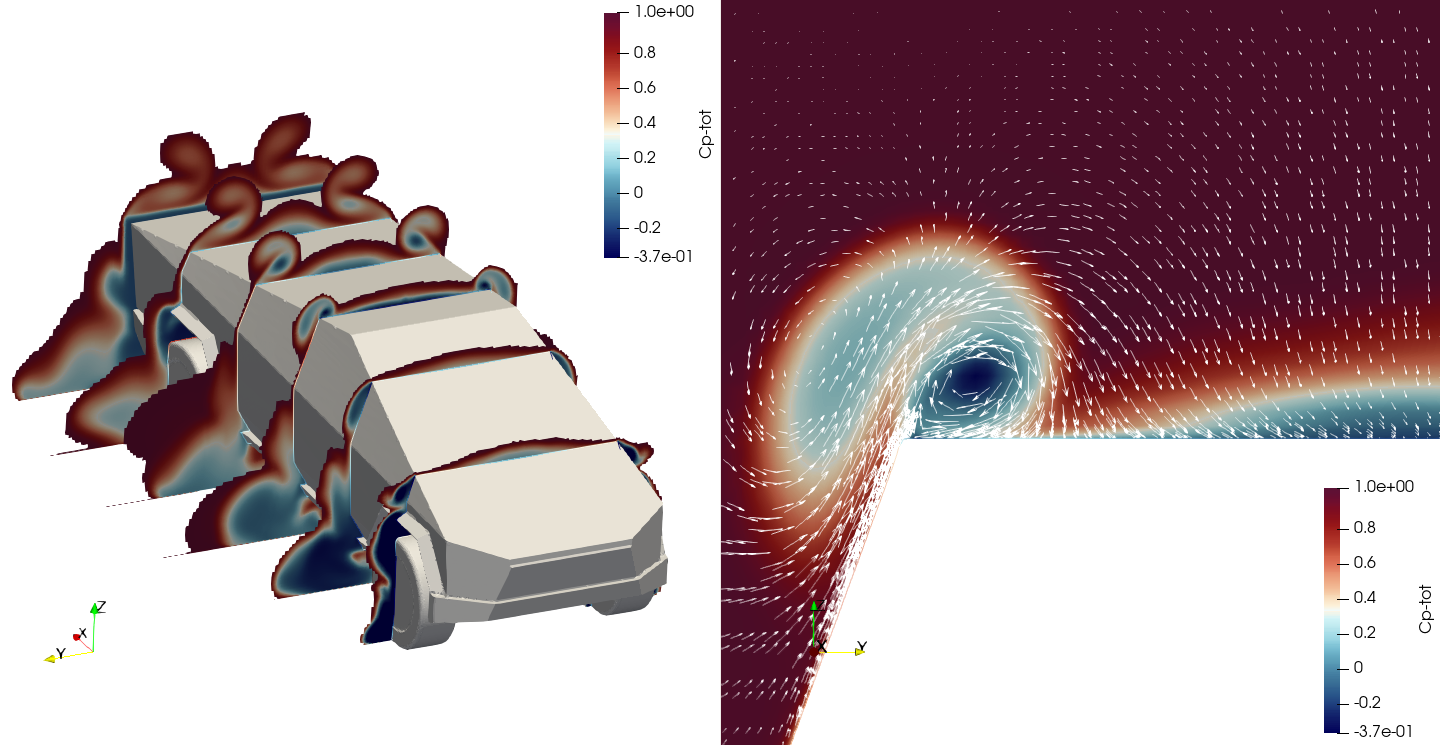
\includegraphics[width=0.9\columnwidth]{vortexes.png}
  \caption{Slice and contour visualizations: blue regions represent vortexes' nuclei, lower zone pressure.\label{vortexes}}
\end{figure}
\subsection{Discussion}
Those vortexes induce a quick reattachment of the flow upon the roof. As it happens on delta wings ~\ref{delta}, the geometry induces a flow separation that results in vortexes that push the flow onto the surface. The tapered shape of the vehicle toward the roof enhances vortexes development. 
\begin{figure}[htp]
  \centering
  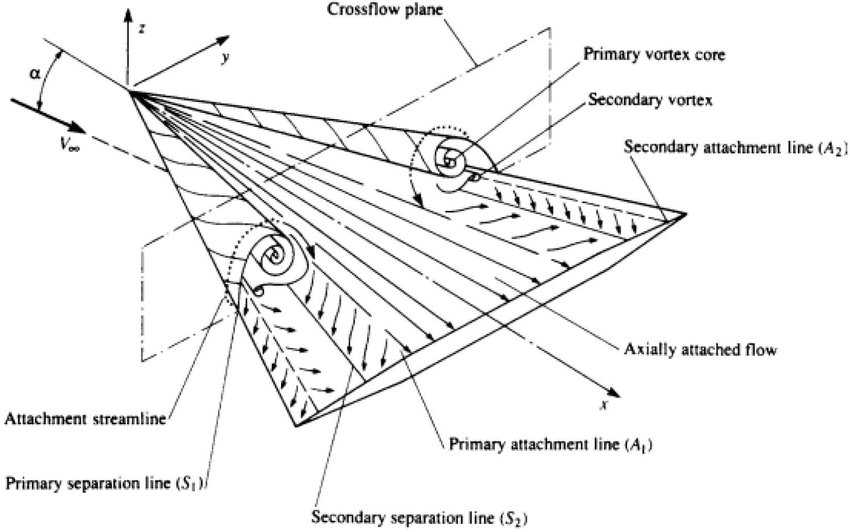
\includegraphics[width=0.9\columnwidth]{delta.jpg}
  \caption{Phenomenology of a delta wing.\label{delta}}
\end{figure}
As emerges from a comparison with the \emph{Wagon} type, the larger angle between the windshield and the roof, reduces the recirculation zone at the corner ~\ref{sloped&wagon}. In spite of that, vortex development is affected and a lower intensity is observed. More importantly, the wake is pretty much affected: the horizontal roof leads to a poor pressure recovery. Instead, the sloped roof of the \emph{Sloped} type, leads the wake to close tighter and sooner: this entails a lower $C_x$.
\begin{figure}[htp]
  \centering
  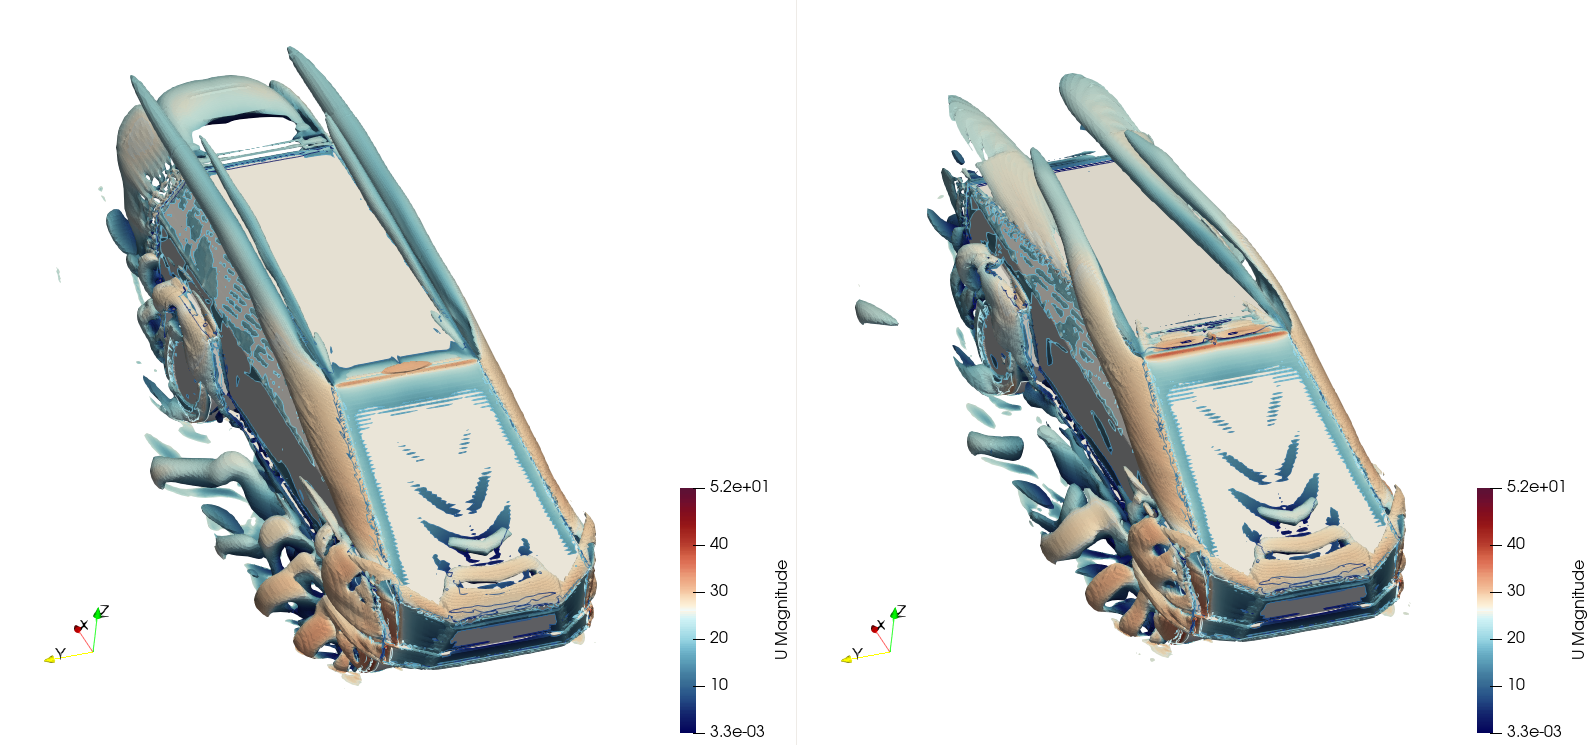
\includegraphics[width=0.9\columnwidth]{sloped&wagon.png}
  \caption{Vortex intensity decreases for an horizontal roof.\label{sloped&wagon}}
\end{figure}
Between full-scale and wind tunnel cases, minor differences in the coefficients is observed, exception made for the pickup. That difference is attributable to a large separated region in the open-cargo area due to which, in this case, the symmetry assumption fails.
An experimental campaign was lead in order to validate CFD results. 
\section{Wind tunnel}
\subsection{CAD adjustments and 3D printing}
Wind tunnel testing required a slightly different CAD: the to-be-printed model had to meet both the 3D printing and the wind tunnel requests. 
Only the \emph{Pickup} model was designed to be printed, since the \emph{Sloped} and \emph{Wagon} ones could be obtained by covering the cargo area with a sloped and a horizontal-top, respectively  ~\ref{assembly}.
Furthermore, the model had to be constrained to the iron plate connected to the balance. Therefore, a recess in the belly of the car was realized.
The model was printed with Fused Deposition Molding. Due to the limited volume of the printer chamber, it had to be split into three portions (front, central, rear) that would be assembled by means of pin joints.
In order to investigate ground-clearance effect, the tyres needed to be displaced upward and downward to accomplish the different heights of the vehicle. A set of three holes was therefore realized for each tyre housing, where to insert the tyre axle. Tyres and covers were printed separately. 
\begin{figure}[htp]
  \centering
  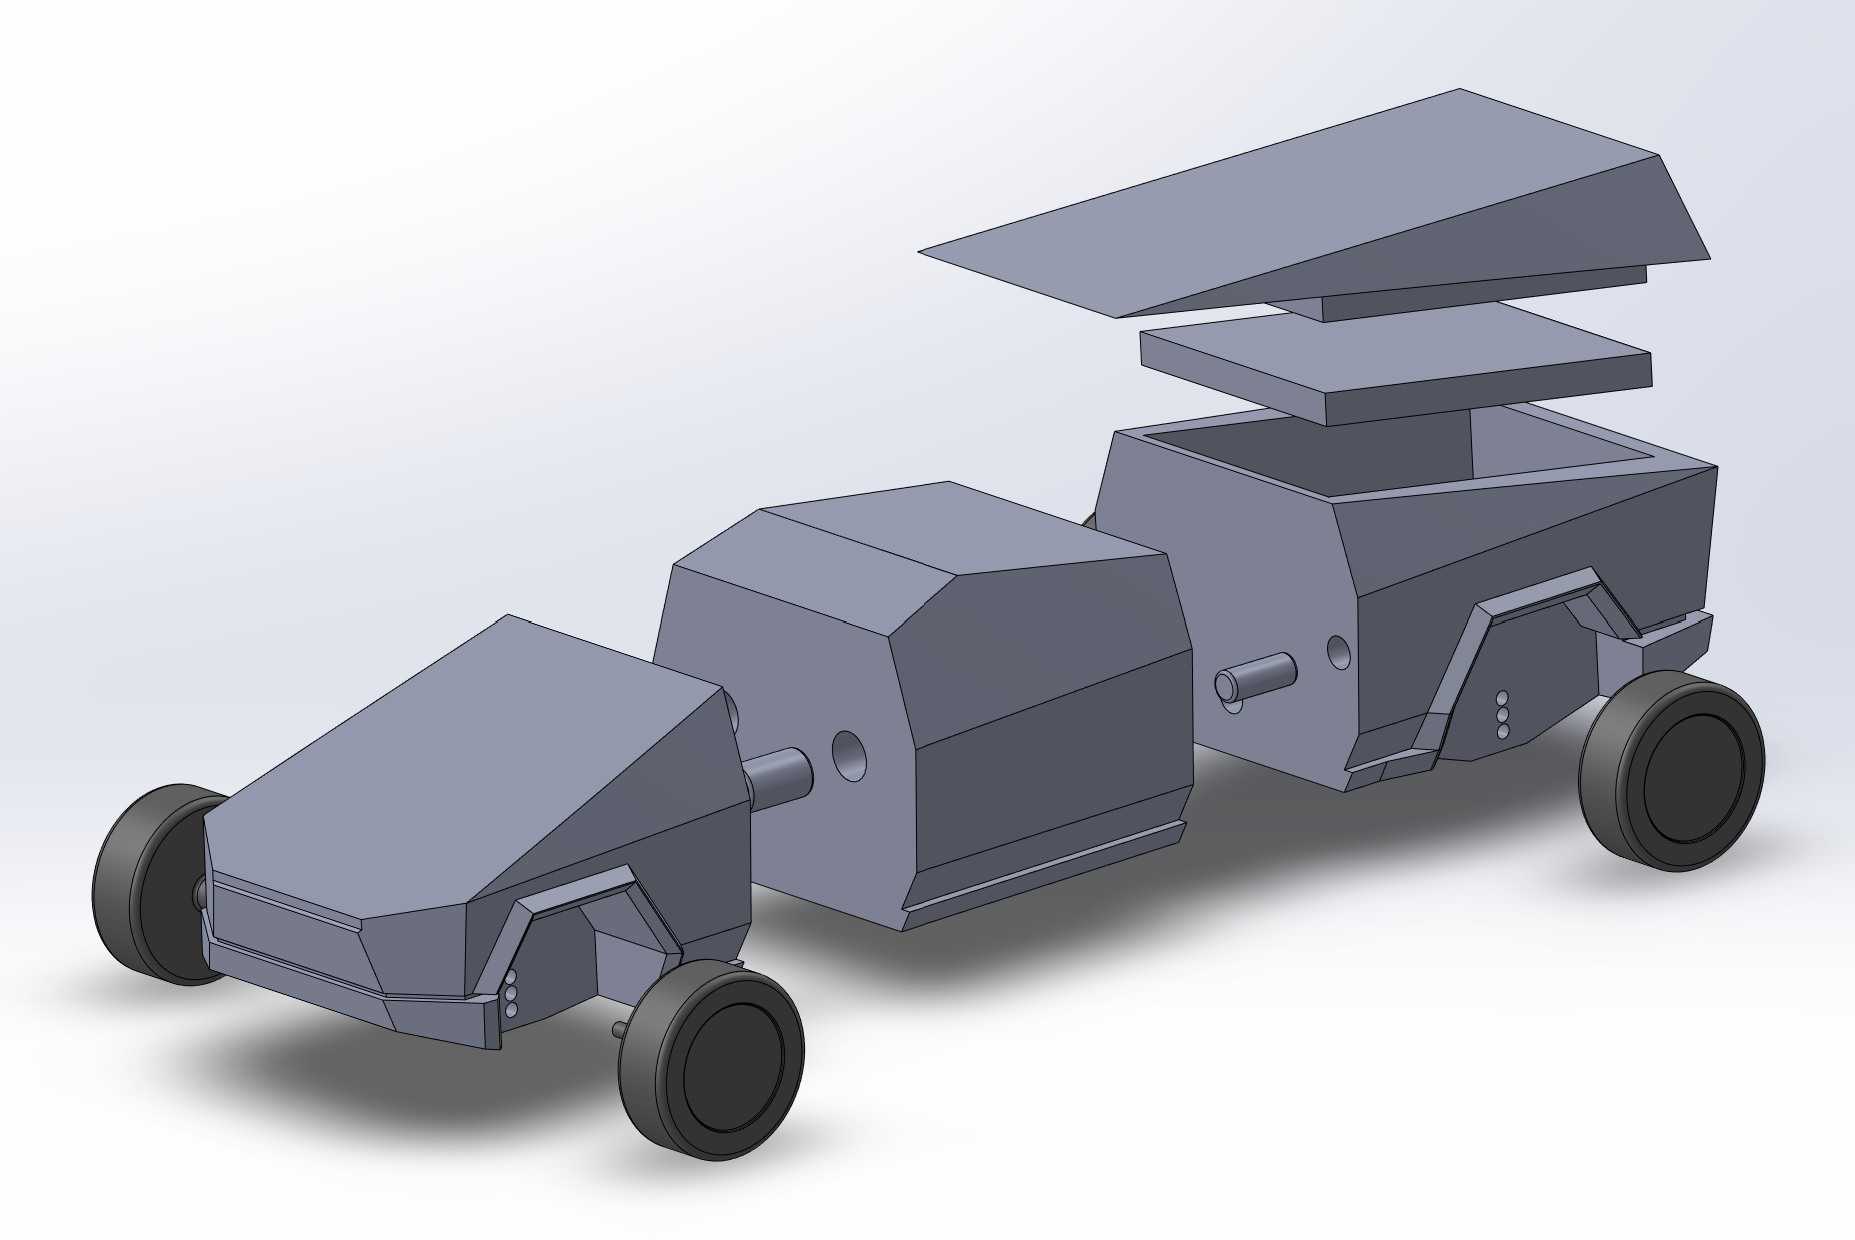
\includegraphics[width=0.9\columnwidth]{assembly.png}
  \caption{Assembly of the model.\label{assembly}}
\end{figure}
The scale of the model had to meet two constraints. The recess could not be split between two portions, for this could have affected the fitting on the balance plate. The maximum blockage ratio for the wind tunnel was limited to 2,51\% \cite{Blockage}. Hence a 1:16 scale was chosen. 
\subsection{Experimental setup}
\subsubsubsection{Motor} The fan was punt into motion by an electric driver, capable of producing a maximum air flow of approximately 20 $m/s$. An inverter allowed to regulate the flow.
\subsubsubsection{Test section} The test section measures 1x0.5x0.5 $m$ (LxWxH).
The speed in the test section is measured with a Pitot Tube connected to a manometer which provides the differential pressure with respect to the ambient. The wind velocity is carried out with the steady-state incompressible Bernoulli theorem, applied to test section conditions with respect to ambient ones.
FORMULA!!
$u=√((2*(p_amb-p_test))/ρ)$
    \begin{figure}[htp]
      \centering
      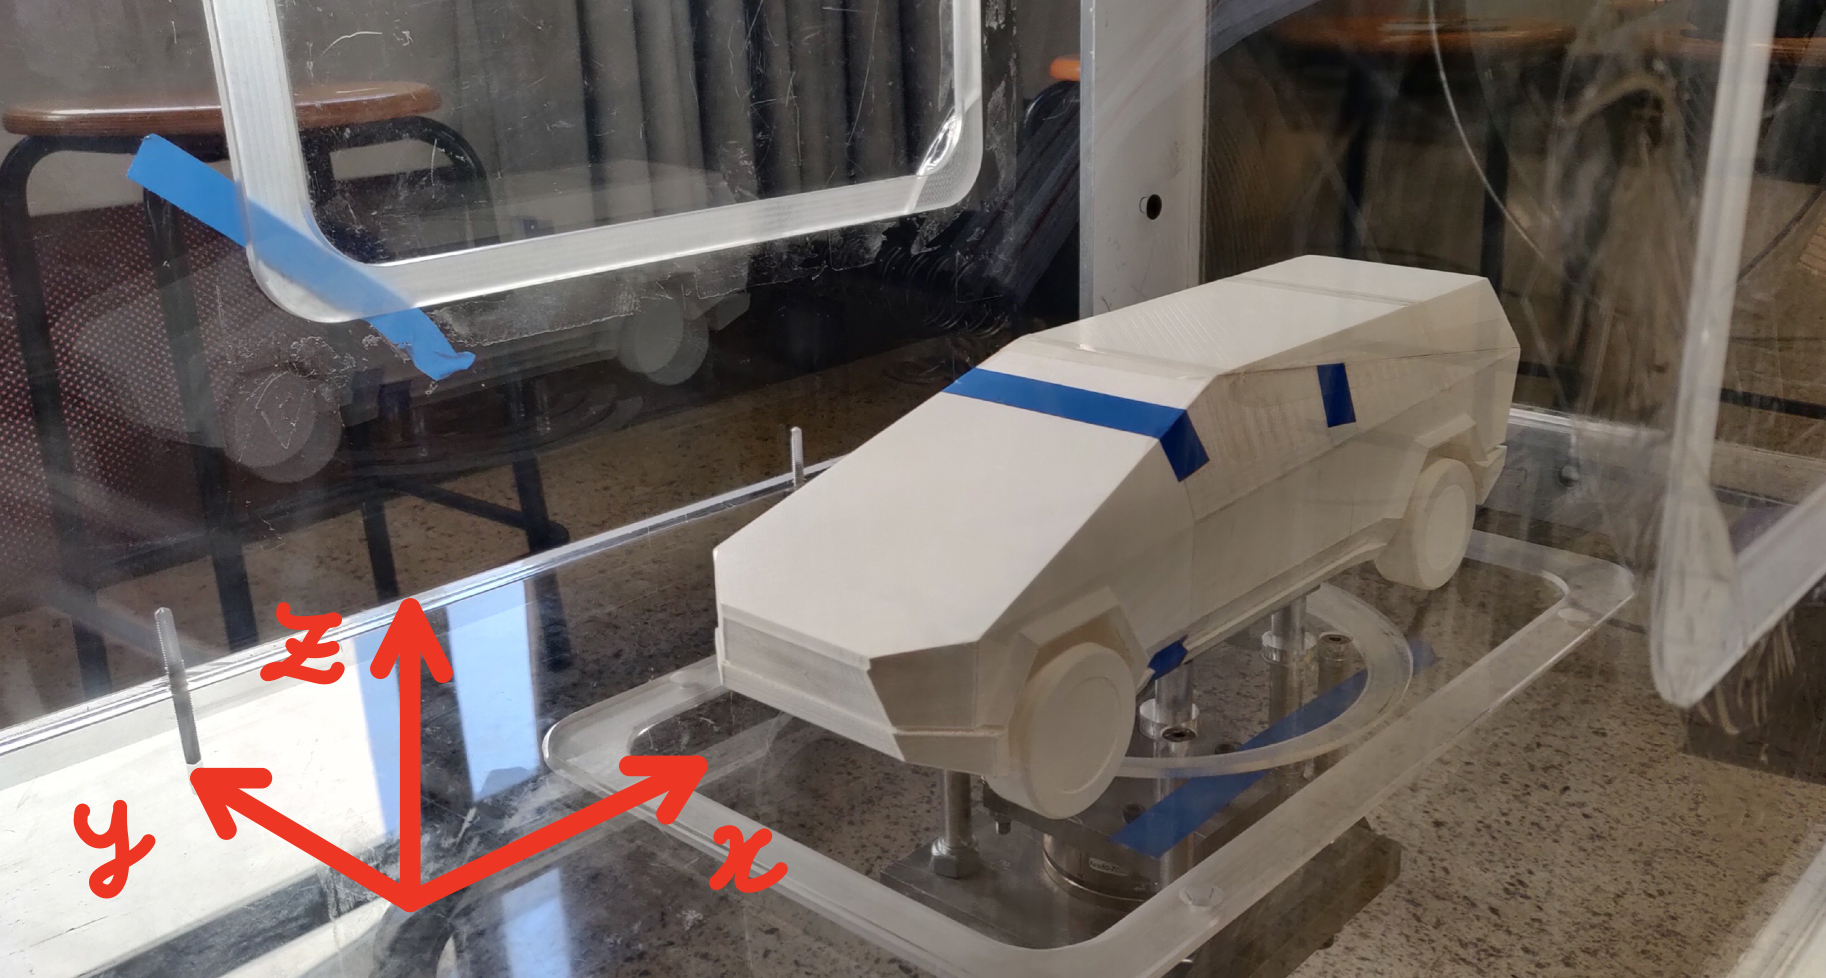
\includegraphics[width=0.9\columnwidth]{windtunnel.jpg}
      \caption{Vortex intensity decreases .\label{windtunnel}}
    \end{figure}
\subsubsubsection{The balance.} The force balance is placed underneath the test section. An iron plate mechanically connected to the balance allows the model to be constrained to it. 
\subsection{Testing}
The same tests were performed for each configuration. First, considering zero yaw angle, the model was tested at four wind velocities: 5, 10, 15, and 20 $m/s$. The three vehicle heights were studied for each velocity and configuration. 
Then, the yaw angle was changed at maximum wind velocity and nominal height for each configuration. Six yaw angles were tested: 5°, 10°, 15°, 30°, 60°, 90°. 
Data collection has been performed over a time window of one minute for each measurement.
\subsection{Data processing}
$C_x$, $C_l$, $C_m$ where sought.The data have been averaged along the time window and then linearly interpolated to obtain the coefficients behaviour
\subsubsubsection{Approximations.} During the testing, many sources of error have been run into: uncertainty of the measure instruments (balance, manometer), maximum velocity provide-able by the driver, mechanical vibrations induced by fan motion, precision in model fitting (model constraint on the balance plate, yaw angle measuring and setting), Bernoulli theorem hypothesis matching (steady state). All these error sources add up, making non-reliable the experimental results.A tailored uncertainty estimation and propagation analysis should be performed in order to take into account the error propagation of the data. 
However, the collection of experimental data still have its relevance, namely, in the trend of the quantities, and not in the single value itself. That's why its analysis is hereby presented.
\subsection{Results}
\subsubsubsection{$C_D$.}The $C_D$ has been computed by adimensionalising the drag force with respect to the frontal area of the model, equal to 3,22 $m^2$. Hence the drag coefficient is computed with respect to the vehicle reference, and it's called $C_x$ \\
$C_x$=$F_x$/$(1/2 ρu^2 A)$ 

\begin{figure}[htp]
      \centering
      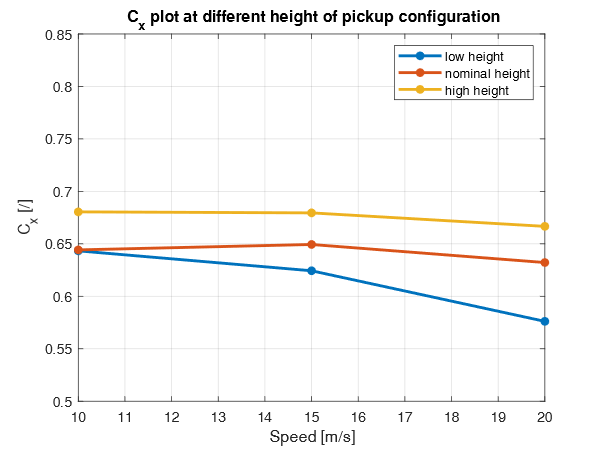
\includegraphics[width=1\columnwidth]{cxpickup.png}
      %\caption{$C_x$ behaviour for varying velocities at different heights.\label{}}
    \end{figure}
    \begin{figure}[htp]
      \centering
      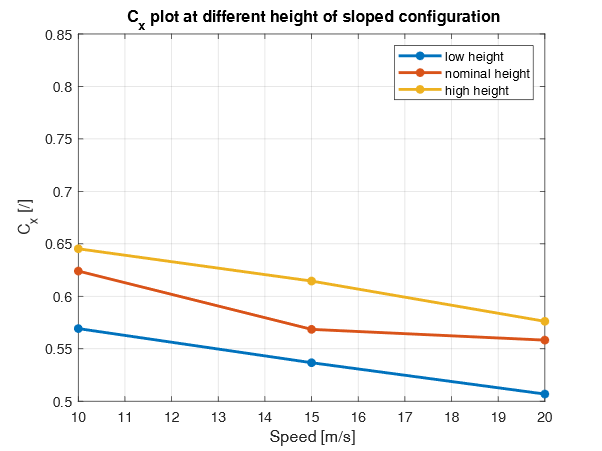
\includegraphics[width=1\columnwidth]{cxsloped.png}
      %\caption{$C_x$ behaviour for varying velocities at different heights.\label{}}
    \end{figure}
    \begin{figure}[htp]
      \centering
      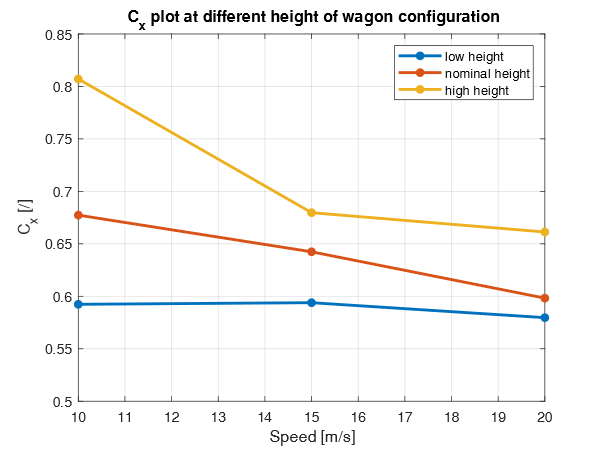
\includegraphics[width=1\columnwidth]{cxwagon.png}
      \caption{$C_x$ for the three configurations at for varying velocities and height.\label{}}
    \end{figure}
    
\subsubsubsection{$C_L$.} The measurement of the lift coefficient were affected by a major error: its data have been omitted due to lack in physical correspondence.
\subsubsubsection{$C_m$.}A study about the overturning moment has been done in order to assess the influence of the tail shape in crosswind condition. The Cm was computed with respect to the axis through the contact points of the downwind tyres \ref{bracci}. To do so, a transport moment has to be added to the rolling moment, due to the contribution of the forces Fy and Fz, measured at the balance.

\begin{figure}[htp]
        \centering
        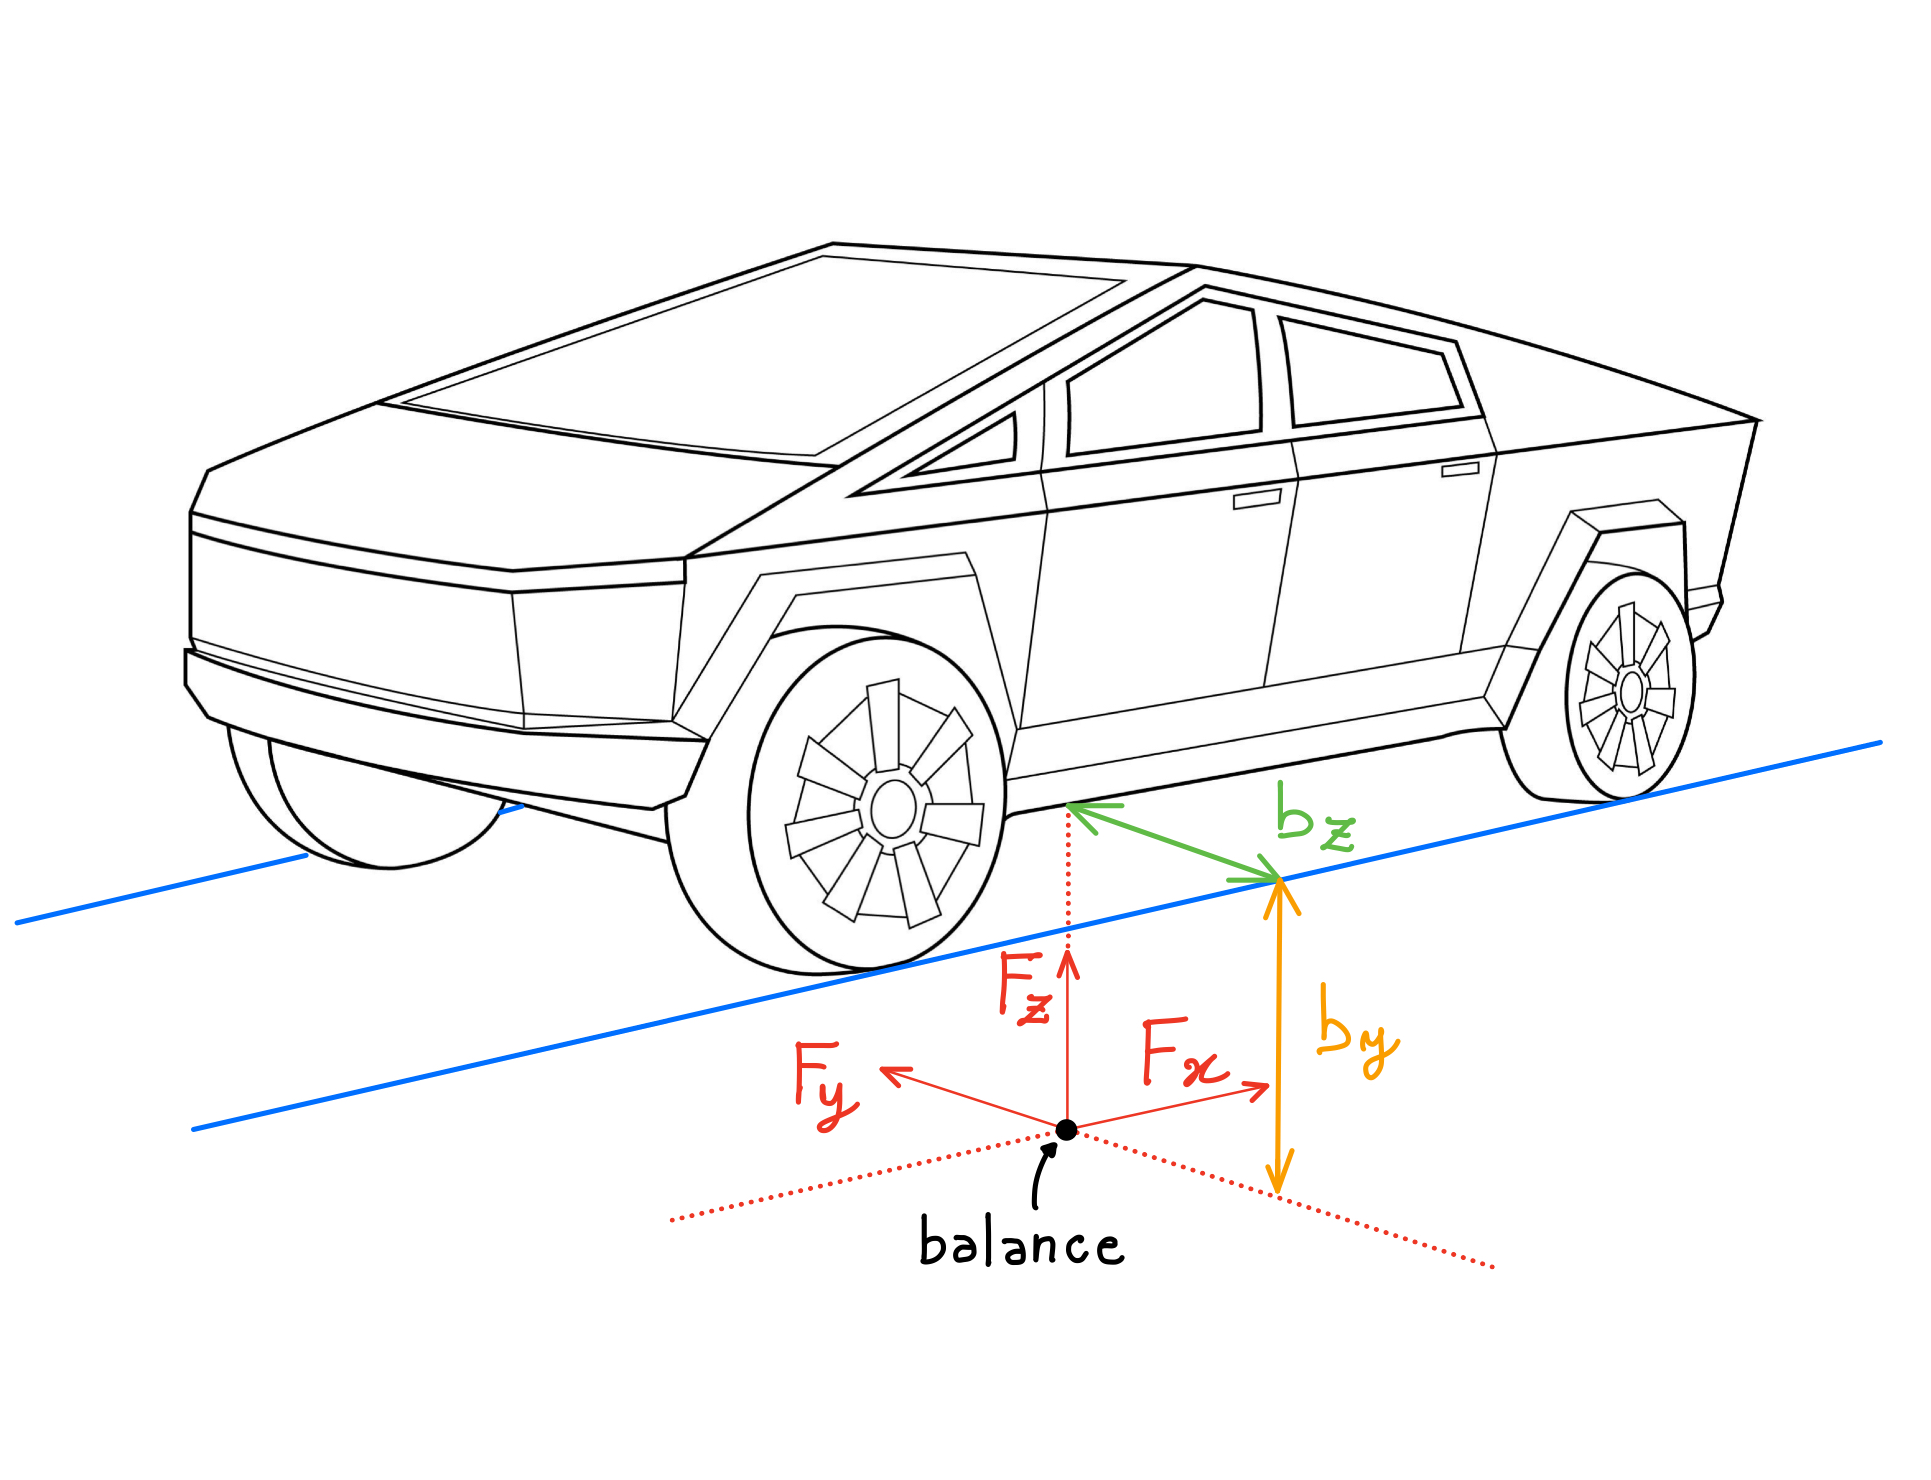
\includegraphics[width=1\columnwidth]{bracci.png}
        \caption{$F_y$ and $F_z$ transport affects the $C_m$.\label{bracci}}
    \end{figure}
$M=M_x+F_y*b〖+F〗_z*s$
$C_m=M/(1/2 ρu^2 A*l)$
Where $l$ is the car width. $C_m$ behaviour at varying yaw angles for different configurations is shown in figure \ref{cm}
\begin{figure}[htp]
        \centering
        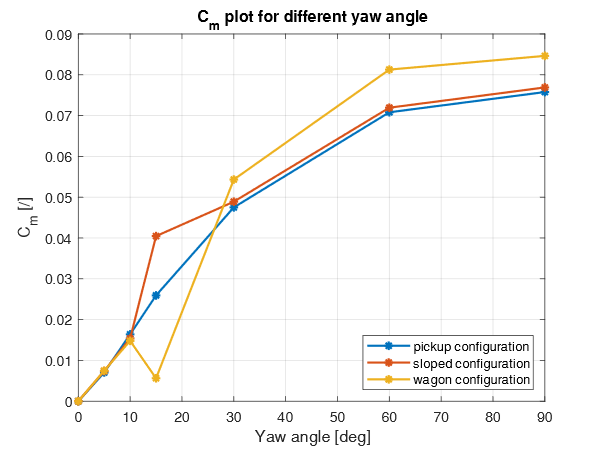
\includegraphics[width=1\columnwidth]{cm.png}
        \caption{$C_m$ for different yaw angles.\label{cm}}
    \end{figure}
\subsection{Discussion}
\subsubsubsection{$C_x$.}The decreasing trend of the coefficients with higher velocities is attributable to the Reynolds effect, for which a drag crisis occurs in a certain range of Reynolds number. In fact, for the range of velocities considered ($u = 20$ $m/s$) and characteristic length of the model ($4*10^-1$ $m$), the order of magnitude of the Reynolds number is $10^5$, thus we are near to the drag crisis for a bluff body \cite{dragcrisis} \ref{dragcrisis}.
    \begin{figure}[htp]
        \centering
        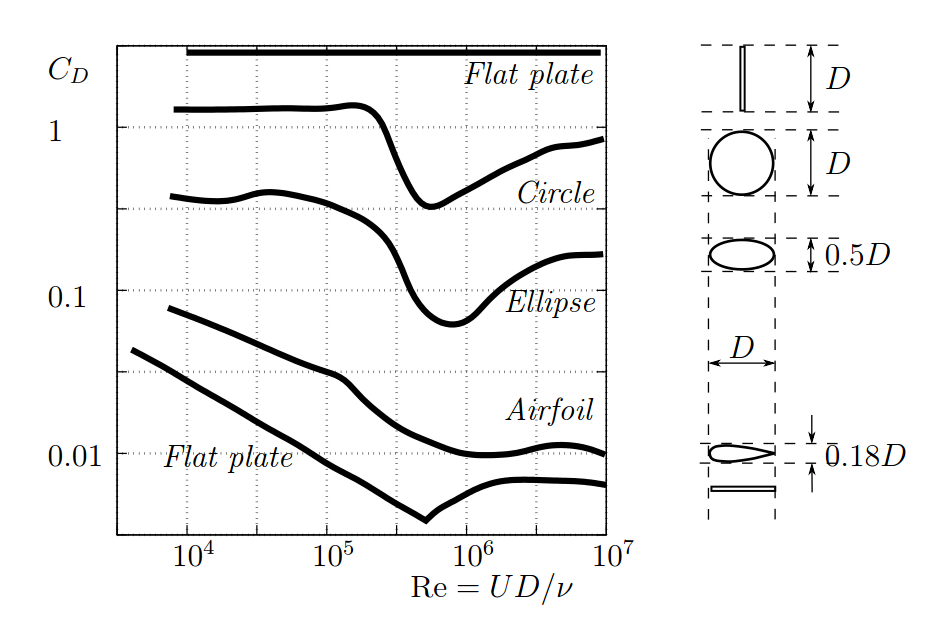
\includegraphics[width=1\columnwidth]{dragcrisis.png}
        \caption{Drag coefficient fall for $Re$ around $10^5$ for bluff bodies.\label{dragcrisis}}
    \end{figure}
Differently from what expected \ref{ground}, by lowering the height of the vehicle no drag increase takes place. 
\begin{figure}[htp]
        \centering
        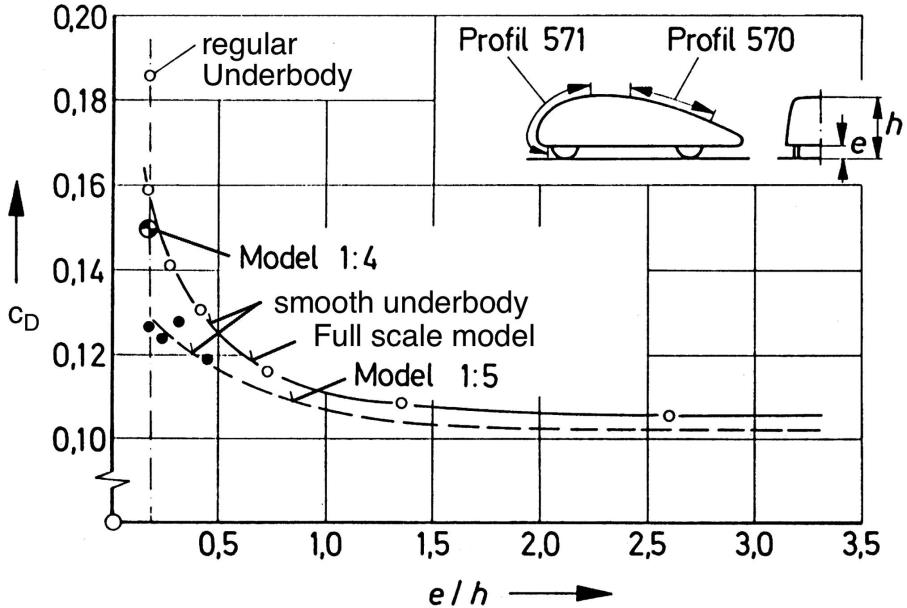
\includegraphics[width=1\columnwidth]{ground.png}
        \caption{Drag coefficient decrease for for wing-like bodies close to the ground.\label{ground}}
    \end{figure}
This is attributable to the fact that the car model is pretty different from a flying-body profile. Furthermore, the resistance of the plate supports becomes more important as the vehicle height increases. 
\subsubsubsection{$C_m$.}The highest values of $C_m$  observed for the configuration with maximum resistant area, namely, the \emph{Wagon} type.
\subsection{Flow visualization}
In order to study the flow attachment around the model, a tuft flow visualization has been performed. The wool tufts were taped to the model surfaces nearby the vortexes influence region, shown by the CFD analysis. 
\begin{figure}[htp]
        \centering
        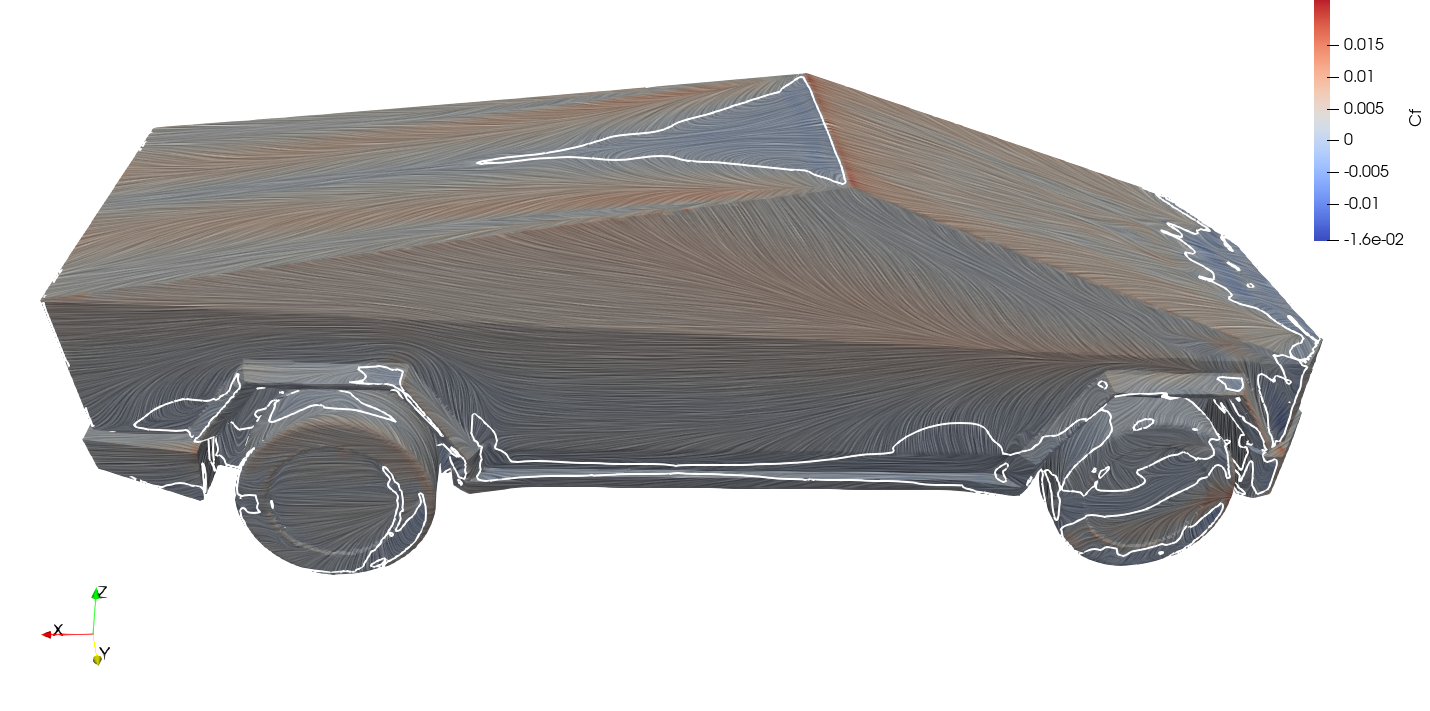
\includegraphics[width=1\columnwidth]{tufts2.png}
        \caption{Flow visualization for CFD.\label{tufts2}}
    \end{figure}

\begin{figure}[htp]
        \centering
        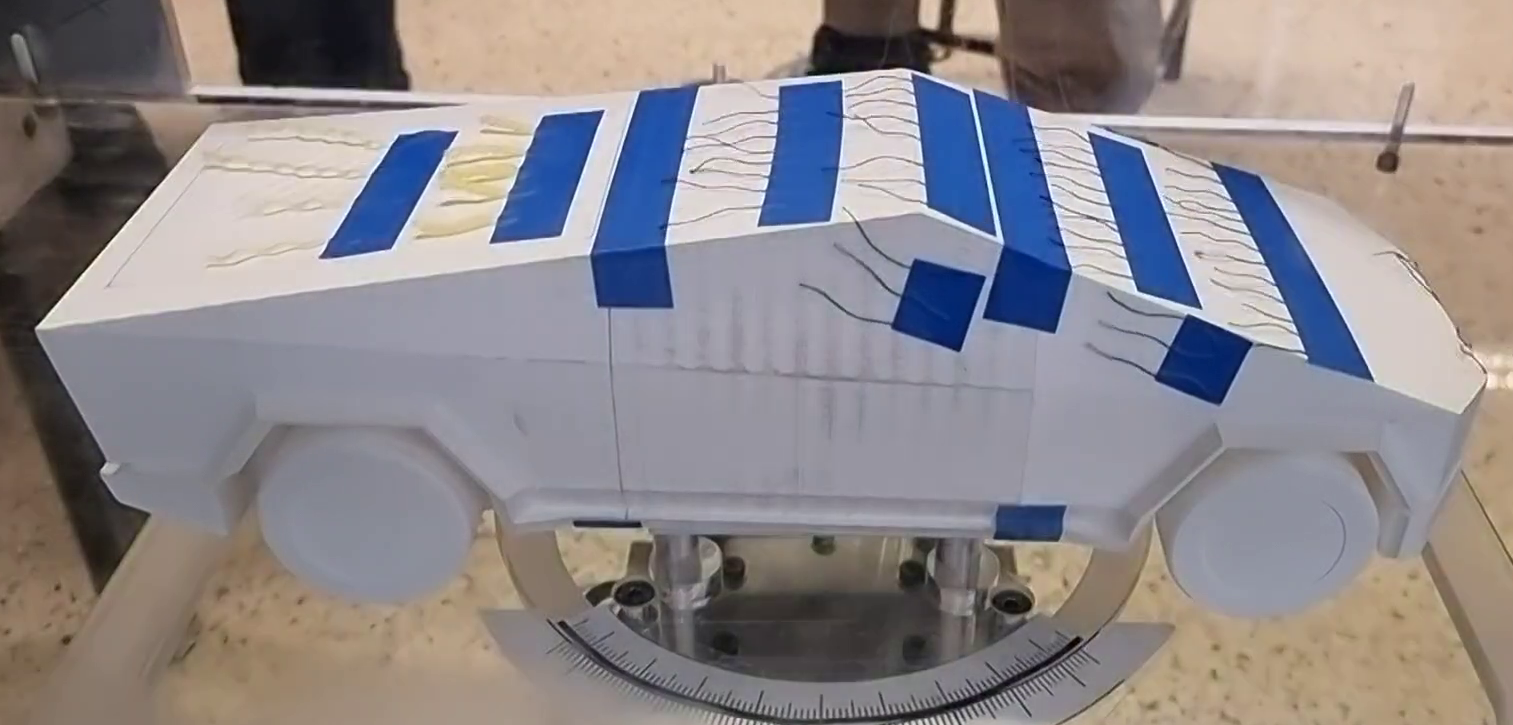
\includegraphics[width=1\columnwidth]{tufts1.png}
        \caption{Flow visualization for wind tunnel.\label{tufts1}}
    \end{figure}
The effect of vortexes can be visualized on the sloped sides \ref{tufts1}: the air flows on the side windows of the car towards the roof. The white-contoured regions in the CFD flow visualization \ref{tufts2} represent the recirculation regions, namely, where the separations take place. There is agreement between the two models: the flow reattaches upon the vehicle roof, and this is due to the presence of counter-rotating vortexes generated at the A and C pillars.
\section{Consumption analysis}
The purpose of this section is to compare the power consumption of the three configurations of the Cybertruck.
The analysis is carried out with the Worldwide Harmonized Light-Duty Vehicles Test Procedure ruled by EU (WLTP). This is a global, harmonized standard procedure for assessing the performances of light-duty road vehicles in terms of fuel consumption, pollutant levels and CO2 emissions.

The total resistance for a car could be considered as a sum of slope, rolling and aerodynamic resistances. The latter depends linearly on the $C_x$, and quadratically on velocity. 

\begin{math}
     R_aero=  1/2 rho C_xSv^2
\end{math}
   

The cycle considers a time window of 1800 seconds during which the car speed is constant. The maximum  speed of the cycle is about 130 km/h and the average speed is 46.5 km/h. The consumption and relative consumption of the three car configurations are listed below.\\

\begin{tabular}{|l|r|r|r|}
\hline
                    &  Sloped   & Pickup    & Wagon \\
\hline
$C_x$ CFD	            & 0.435	    & 0.457	    & 0.502 \\
\hline
Δ$C_x$	        & /	        & 5\%	    & 15\% \\
\hline
Cons. WLTP ($km/kWh$)	& 6.60	& 6.52    & 6.36 \\
\hline
ΔCons. WLTP ($km/kWh$)  & /	    & 1.21\%	& 3.64\% \\
\hline
Cons. 130 k/h ($km/kWh$) & 3.8 & 3.68 & 3.47 \\
\hline
ΔCons. 130 km/h &    / & 3.07\% & 8.75\% \\
\hline

\end{tabular}
			
\section{Conclusions}
In this study the aerodynamic performance of the Tesla Cybertruck is assessed by means of drag and moment coefficients. The geometry of the vehicle induces a flow separation that results in two couples of vortexes that are born at the A and C pillars. Their induction cause the flow to reattach to the surface. The lowest drag coefficient is obtained for the \emph{Sloped} type: $C_x$=0.435 and $C_x$=0.507 according to CFD and experimental analysis respectively. Hence an error of 14\% is obtained between the two. The consumption analysis shows how covering the cargo area of the truck could increase the car autonomy, yet not much difference is spot with respect to the \emph{Pickup}. 

\newpage
\nocite{*}
\printbibliography
\end{document}
